\documentclass{article}

\usepackage[a4paper, margin=1in]{geometry}
\usepackage[onehalfspacing]{setspace} % Correct 1.5 line spacing

\usepackage{graphicx}  % Figures
\graphicspath{{./figures/}}

\usepackage{url}
\usepackage[pdfusetitle]{hyperref}
\usepackage{titlesec}      % Modify title/section/chapter commands
\usepackage{mathtools}     % Various maths related commands
\usepackage{gensymb}       % \degree symbol
\usepackage[thinc]{esdiff} % Derivatives
\usepackage{booktabs}      % \toprule, etc., in tables
\usepackage{doi}           % support DOI links in bibliography
\usepackage{wrapfig}       % figures in text

\usepackage{fontspec}      % Fonts
\usepackage{helvet}
\usepackage{newpxtext,newpxmath}
\defaultfontfeatures{Scale=MatchLowercase, Ligatures=TeX}

% SI units
\usepackage{siunitx}
\sisetup{separate-uncertainty=true,number-mode=text,detect-weight=true}
\DeclareSIUnit\belm{Bm}
\DeclareSIUnit\belw{BW}
\DeclareSIUnit\beli{Bi}
\DeclareSIUnit\belz{BZ}

% https://tex.stackexchange.com/a/43009
\DeclarePairedDelimiter\abs{\lvert}{\rvert}%
\DeclarePairedDelimiter\norm{\lVert}{\rVert}%

% Caption figures
\usepackage{caption}
\DeclareCaptionFont{captionlabelfont}{\bfseries \sffamily}
\DeclareCaptionFont{captiontextfont}{\sffamily}
\captionsetup{labelfont=captionlabelfont, textfont=captiontextfont}

% Change footnote style
\renewcommand{\thefootnote}{\fnsymbol{footnote}}

% Fancy header/footer
\usepackage{fancyhdr}
\pagestyle{fancy}
\renewcommand{\sectionmark}[1]{\markright{\thesection . #1}}
\fancyhf{}
\lhead{\fancyplain{}{\thepage}}
\rhead{\fancyplain{}{\textit{\rightmark}}}

% Bibliography
\usepackage[backend=biber, style=ieee, natbib=true,
			url=false, isbn=true, doi=true,
			eprint=false, urldate=long]{biblatex}
%\addbibresource{references-old.bib}
\addbibresource{references.bib}

% biblatex IEEE style leaves empty parentheses when there is no date/year field.
% Since there are no date fields for many online resources, we use
%   https://tex.stackexchange.com/a/151264
% to stop these parentheses from being generated if there is no date field.
\usepackage{xpatch}
\xpatchbibdriver{online}
{\printtext[parens]{\usebibmacro{date}}}
{\iffieldundef{year}
	{}
	{\printtext[parens]{\usebibmacro{date}}}}
{}
{\typeout{There was an error patching biblatex-ieee (specifically, ieee.bbx's @online driver)}}

\renewcommand{\descriptionlabel}[1]{\hspace*{\labelsep}\spacedlowsmallcaps{#1}}

\titlespacing*{\chapter}{0pt}{1\baselineskip}{1.2\baselineskip}
\titlespacing*{\section}{0pt}{1.25\baselineskip}{1\baselineskip} 
\titlespacing*{\subsection}{0pt}{1.25\baselineskip}{1\baselineskip}
\titlespacing*{\paragraph}{0pt}{1\baselineskip}{1\baselineskip}

% Fix for missing µ in siunitx ???
% https://tex.stackexchange.com/a/428215
\sisetup{math-micro=\text{µ},text-micro=µ}

\newcommand\mytitle    {Millimetre-Wave Cloud Profiling Radar}
\newcommand\mysubtitle {Project Report}
\newcommand\myauthor   {180014855}
\newcommand\mydate     {\today}
\newcommand\mymodule   {PH4111}
\newcommand\mywordcount{2300}

\title {\mytitle}
\author{\myauthor}
\date  {\mydate}

%\usepackage[acronym,nonumberlist]{glossaries}
%\usepackage[acronym,nonumberlist]{glossaries-extra}

\usepackage[nopostdot, toc, nogroupskip, nomain, indexonlyfirst, acronym, symbols, style=long4col, stylemods={longextra}, nonumberlist]{glossaries-extra}

\makeglossaries

%\setabbreviationstyle[acronym]{long-short}

\newacronym{ac:daq}{DAQ}{Data acquisition}
\newacronym{ac:simd}{SIMD}{Single instruction, multiple data}
\newacronym{ac:cpr}{CPR}{Cloud profiling radar}
\newacronym{ac:fmcw}{FMCW}{Frequency-modulated continuous wave}
\newacronym{ac:netcdf}{NetCDF}{Network common data form}
\newacronym{ac:openmp}{OpenMP}{Open multi-processing}
\newacronym{ac:adc}{ADC}{Analogue to digital converter}
\newacronym{ac:dds}{DDS}{Direct digital synthesiser}
\newacronym{ac:dft}{DFT}{Discrete Fourier transform}
\newacronym{ac:fftw}{FFTW}{Fastest Fourier Transform in the West}
\newacronym{ac:mkl}{Intel MKL}{Intel Math Kernel Library}
\newacronym{ac:snr}{SNR}{Signal-to-noise ratio}
\newacronym{ac:if}{IF}{Intermediate frequency}
\newacronym{ac:cpi}{CPI}{Coherent processing interval}
\newacronym{ac:cpu}{CPU}{Central processing unit}

%\newglossaryentry{busywaiting}
%{
%	name=formula,
%	description={A mathematical expression}
%}

\glsaddall

\begin{document}

\begin{titlepage}
	\centering
	{
\includegraphics[width=0.3\textwidth]{uos-logo}}
	\par
	{\LARGE\bfseries University of St Andrews\par}
	{\LARGE School of Physics and Astronomy\par}
	\vspace{1.5cm}
	{\huge\bfseries\mytitle\par}
	{\Large\mysubtitle\par}
	\vspace{2cm}
	{\Large\myauthor\par}
	{\large\textbf{Module:} \mymodule\par}
	{\large\textbf{Word count:} \mywordcount\par}
	\vfill
	{\large\today\par}
\end{titlepage}

\begin{abstract}
	Insert abstract here.
\end{abstract}

\tableofcontents

\section{Introduction}

\section{Signal processing theory}
\subsection{FMCW-Doppler radar}
The main 


\begin{figure}
	\centering
	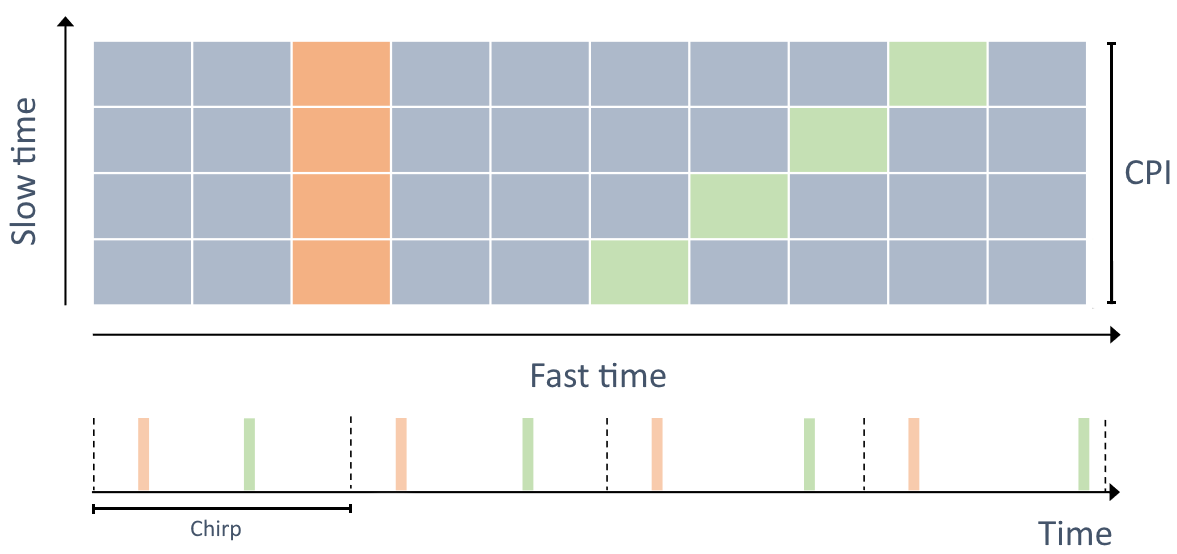
\includegraphics[width=\textwidth]{slow-fast-time}
	\caption{Fast-time vs slow-time. Adapted from \cite{SlowFastTimeFig}.}
	\label{fig:SlowFastTime}
\end{figure}

\subsection{Signal averaging}
\begin{figure}
	\centering
	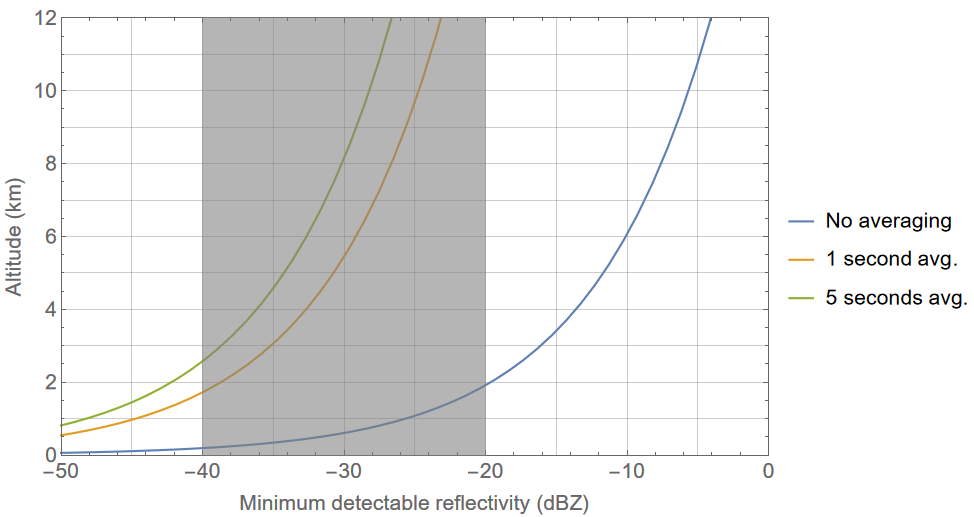
\includegraphics[width=\textwidth]{sensitivity}
	\caption{Radar sensitivity  (Own work).}
	\label{fig:SlowFastTime}
\end{figure}

\subsection{Doppler moments}

\section{Requirements}

\begin{figure}
	\centering
	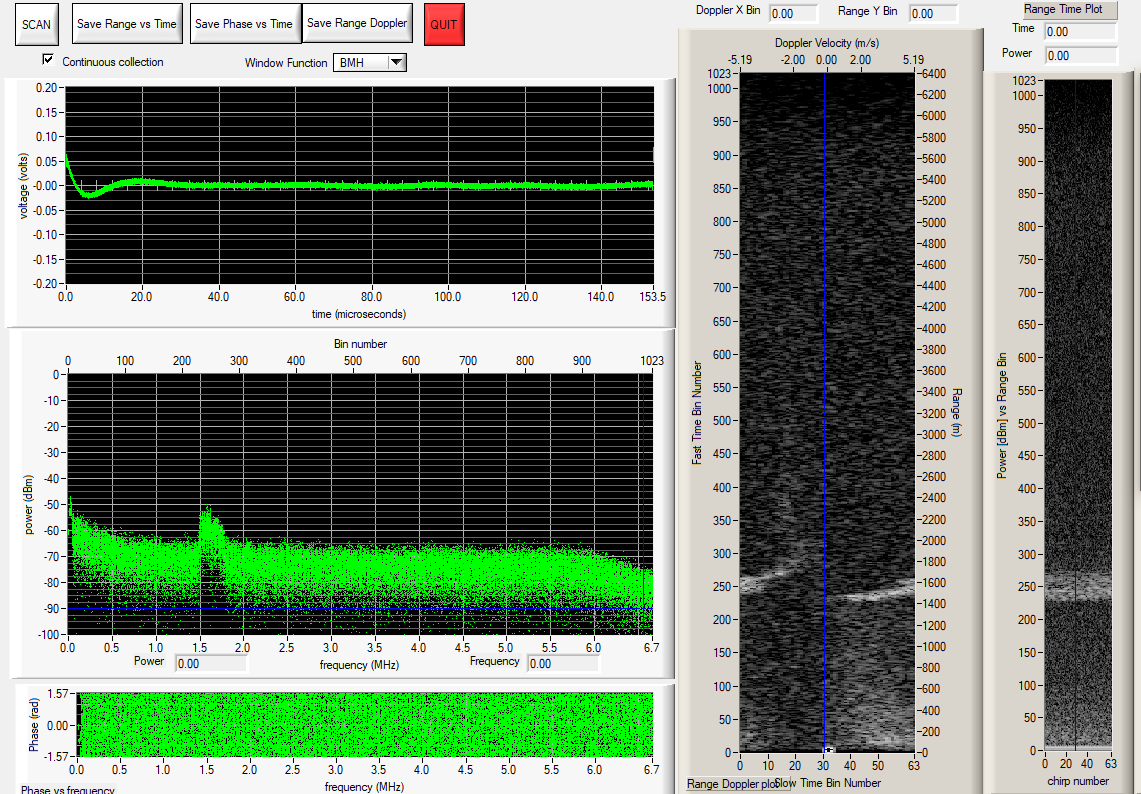
\includegraphics[width=\textwidth]{mark-1-rain}
	\caption{Screenshot of Mark I user interface, taken during precipitation.}
	\label{fig:Mark1Rain}
\end{figure}

\section{Design and implementation}
\begin{figure}
	\centering
	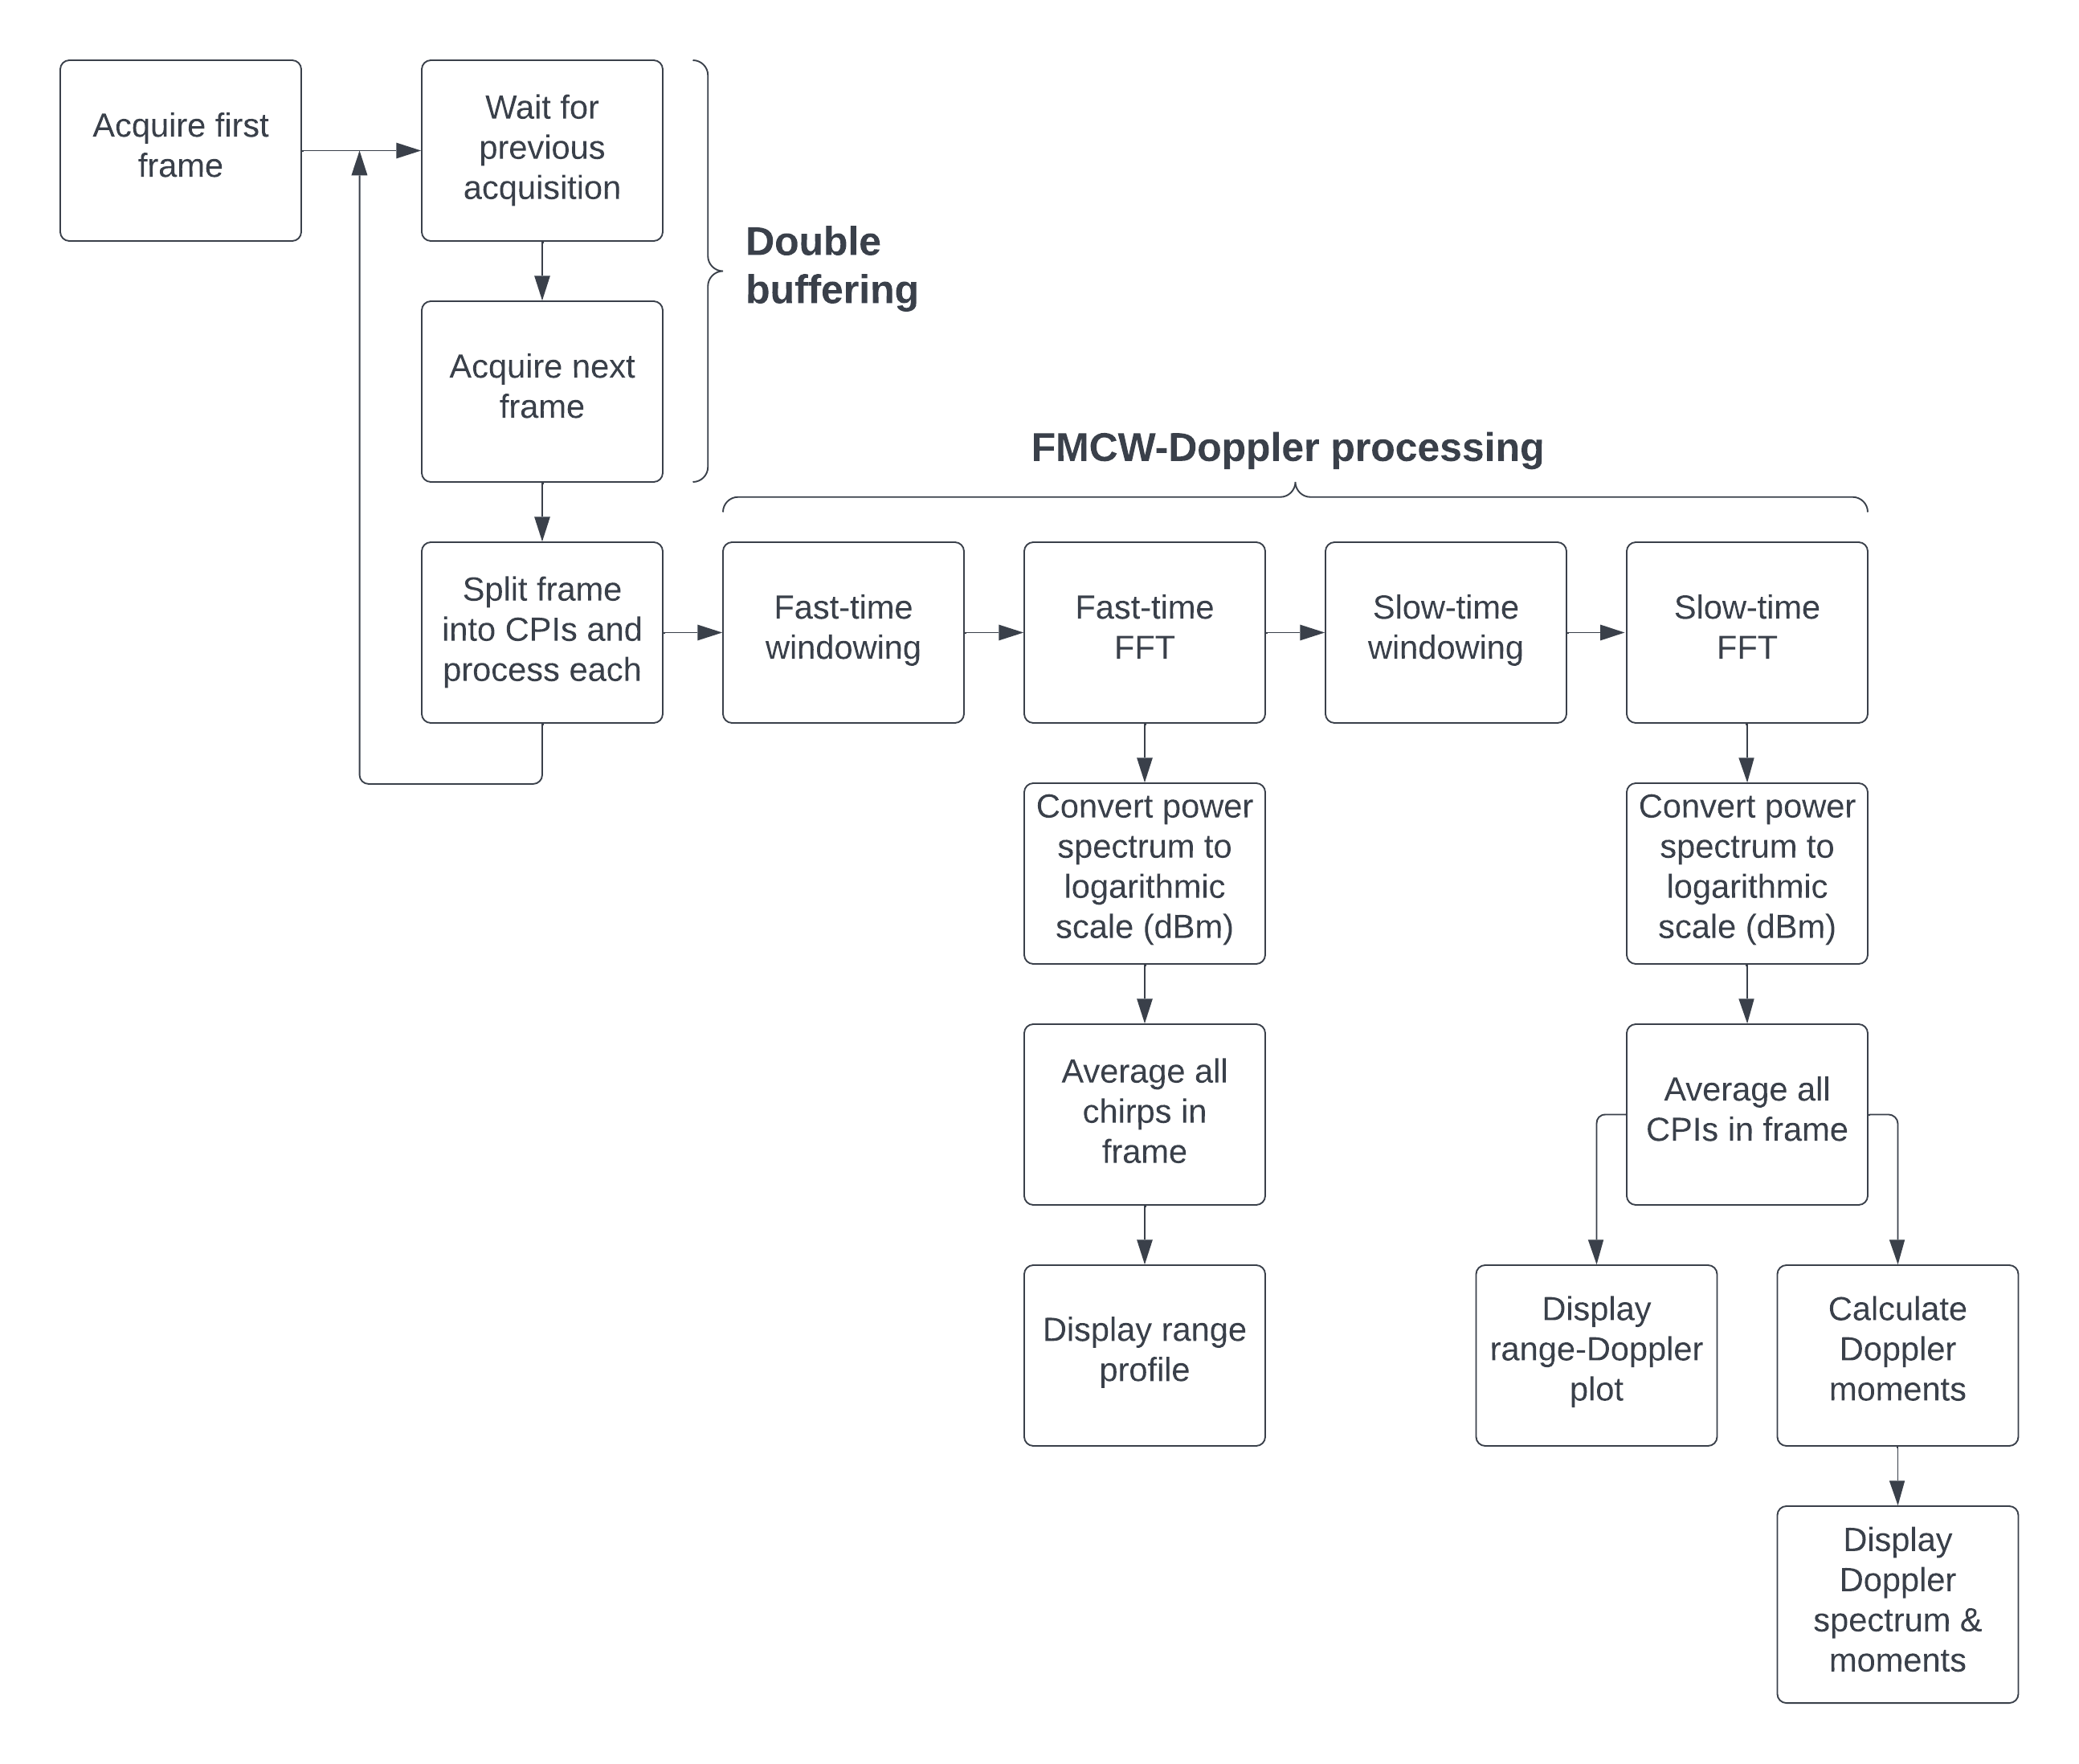
\includegraphics[width=\textwidth]{signal-processing-diagram}
	\caption{Simplified block diagram illustrating key signal processing steps. (Own work)}
	\label{fig:SignalProcessingDiagram}
\end{figure}

\subsection{Data acquisition}
\subsubsection{Double buffering}
To ensure real-time output, a double buffering approach is used.
One buffer is used to store the incoming frame and another stores the previously acquired frame 
While the next frame is being acquired, the most recent frame is processed.

\subsubsection{Alternatives to double buffering}
The approach in Mark II used one acquisition thread and one processing thread. The acquisition thread repeatedly acquires data and appends it to a thread-safe queue, which the processing thread pulls from

The main issue with this approach is the acquisition thread wastes \acrshort{ac:cpu} time waiting for the frame to be acquired and transferred to memory


\subsubsection{Testing}
To facilitate testing the software, a mock implementation of the \acrshort{ac:daq} was created. 

\subsection{FMCW-Doppler processing}


\subsubsection{Testing}

\subsection{Averaging}
\subsection{Doppler moments}

\section{Results}

\begin{figure}
	\centering
	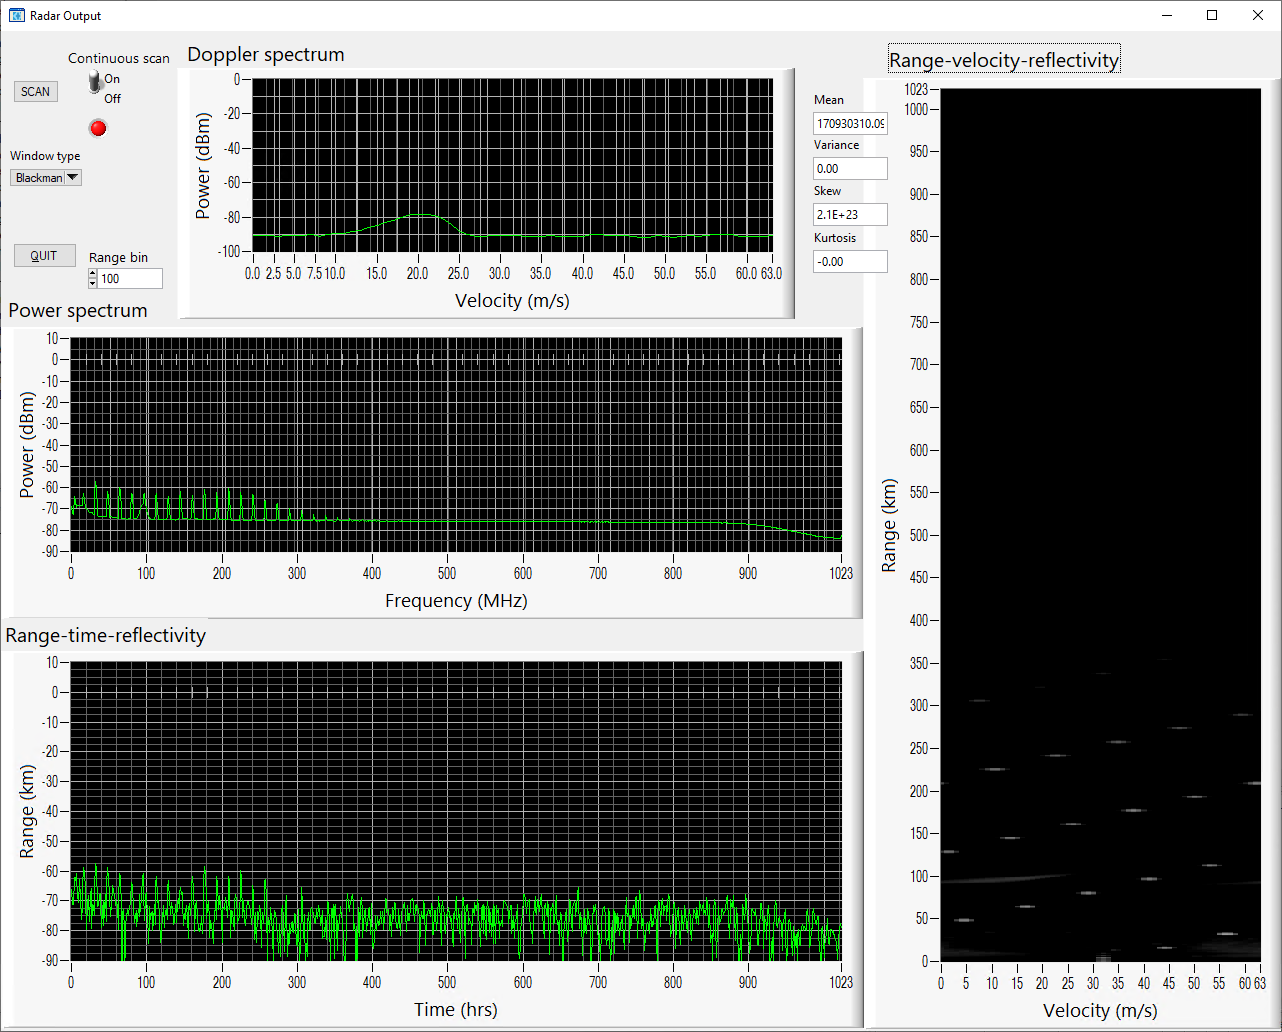
\includegraphics[width=\textwidth]{working-cloud}
	\caption{Screenshot of the new user interface.}
	\label{fig:WorkingCloud}
\end{figure}

\begin{figure}
	\centering
	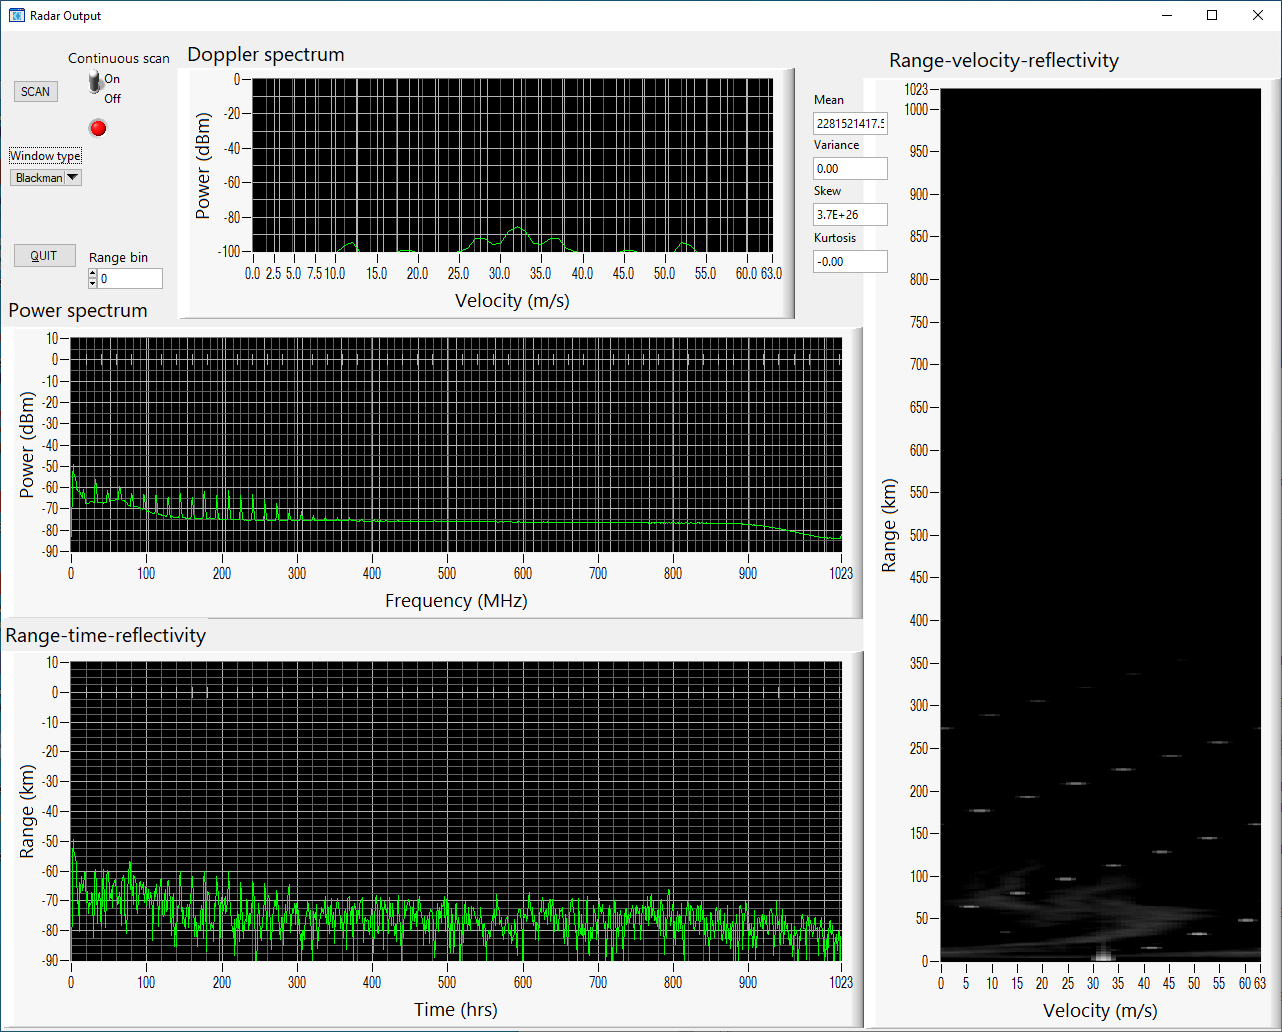
\includegraphics[width=\textwidth]{working-hail}
	\caption{Screenshot of the new user interface, showing hail.}
	\label{fig:WorkingHail}
\end{figure}

\begin{figure}
	\centering
	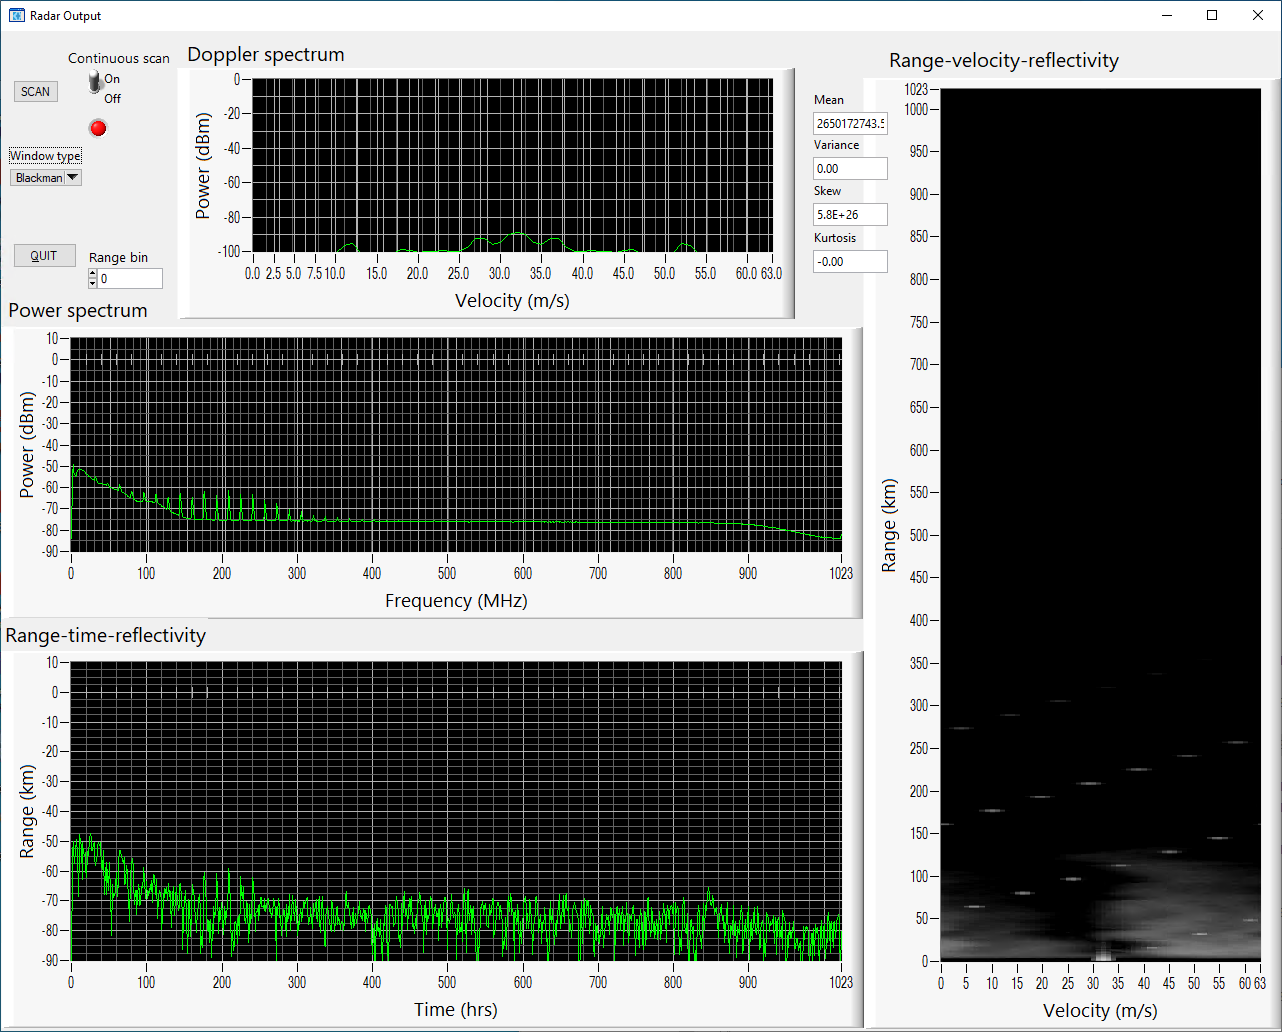
\includegraphics[width=\textwidth]{working-heavy-rain-snow}
	\caption{Screenshot of the new user interface, showing heavy rain and/or sleet.}
	\label{fig:WorkingHeavyRainSnow}
\end{figure}

\subsection{Performance}
Compare processing time of previous software

\section{Future work}
\subsection{Effect of ambient temperature}
\subsection{NetCDF}

\subsection{Performance improvements}
\subsubsection{Multithreading}
\subsubsection{OpenMP}
\subsubsection{SIMD}
Single instruction, multiple data (SIMD) is another type of parallel processing that 

\section{Conclusions}

\clearpage
\printglossary
\printbibliography

\end{document}
